\section{Black Pepper \& Long Pepper}
\label{sec:pepper}

\begin{spice}\label{spice:pepper}
\textsc{Pepper} \hfill \href{https://powo.science.kew.org/taxon/682369-1}{POWO} \\
\textbf{English:} \textit{pepper}; \textit{black pepper}. 
\textbf{Arabic:} {\arabicfont{فلفل}} \textit{filfil, fulful}; {فلفل أسود} \textit{fulful aswad} [black pepper]. 
\textbf{Chinese:} {\traditionalchinesefont{胡椒}} \textit{hújiāo} [barbarian-pepper]; 黑胡椒 \textit{hēihújiāo} [black-barbarian-pepper]. 
\textbf{Hungarian:} \textit{bors} [pepper]; \textit{fekete bors} [black pepper].  \\
\noindent{\color{black}\rule[0.5ex]{\linewidth}{.5pt}}
\begin{tabular}{@{}p{0.25\linewidth}@{}p{0.75\linewidth}@{}}
Plant species: & \taxonn{Piper nigrum}{L.} \\
Family: & \textit{Piperaceae} \\
part used: & fruit \\
Region of origin: & Malabar coast (South India) \\
Cultivated in: & Vietnam; Brazil; Indonesia; India; Sri Lanka; etc. \\
Color: & black; white; green \\
\end{tabular}
\end{spice}

\begin{figure}[!ht]
	\vspace{-4ex}
	\centering
	\subfloat{\includegraphics[width=0.3\linewidth]{imgs/spices/pepper-black-2.jpg}}
	\hfill
	\subfloat{\includegraphics[width=0.3\linewidth]{imgs/spices/pepper-white-penja-2.jpg}}
	\hfill
	\subfloat{\includegraphics[width=0.3\linewidth]{imgs/spices/pepper-green-1.jpg}}
	\caption[True peppers: black, white, and green.]{Black pepper from the Malabar coast in India, white pepper from the Penja Valley in Cameroon, and green peppercorns. \textit{Piper nigrum}. Credits: Aromatiques.}
	\label{fig:pepper_imgs}
\end{figure}

% DESCRIPTION:
Black pepper is the dried fruit (drupe)\footnote{A type of fleshy fruit with thin skin and a single, central pit containing the seed, also known as a ``stone-fruit'' (e.g.: plum, cherry, peach, nutmeg, olive, mango). It is a term used to denote the contrast to a botanical ``berry'', which contains many seeds (e.g.: blueberry, grape).} of the species \textit{Piper nigrum}. Pepper fruits are often called peppercorns, and they come in black, white, green, and even red. However, black pepper\index{pepper!black}, white pepper\index{pepper!white}, green\index{pepper!green} and ``true'' red peppercorns\index{pepper!red} are not different varieties, they are the fruits of the same plant. Their difference merely lies in the harvesting and drying process. All of them have a unique, pungent taste and a fresh, spicy aroma that they release when being crushed or ground. 

% INTRO:
Black pepper\index{pepper|textbf}\index{pepper!black} is the most important, most popular, and most consumed spice in the world \autocite[721]{mabberley_mabberleys_2017}. Valued for its pungency and flavor, pepper has been used since ancient times in traditional medicine and gastronomy from East to West, and it is the most influential spice that shaped human history. It is found and used virtually everywhere around the globe \autocite[253]{hill_contemporary_2004}, and most of us are familiar with the biting sensation it causes on the tongue and in the nose. Black pepper was one of the first aromatic substances used medicinally in India, and one of the first products of global commerce to be traded, alongside long pepper, and ginger. It was transplanted to other tropical regions of Asia early on, and cultivated extensively. Black pepper's early diffusion is remarkably interesting, it is the prototype spice for many of us. Also referred to simply as \textit{pepper} from here on, it was among the first oriental spices to reach the Occident \pvolcite[]{1}[86]{peter_handbook_2012}. Pepper was known to the ancient Egyptians, Greeks, and Romans in the West, and have changed medieval Europe. It was even used as currency in small amounts. Today it accounts for more than a third of all spices traded in the world, making it the most traded spice as well \autocite{ravindran_piper_2017}. Its importance is well demonstrated by the many books and monographs about its history \autocite[see][]{shaffer_pepper_2013,wernick_pepper_2014}, agronomy \autocite[see][]{ravindran_black_2000,nair_geography_2020}, and appeal \autocite[see][]{de_kerros_pepper_2016,barth_pepper_2019}.

% OPERATIVE
\begin{note}
    Throughout this dissertation---unless stated otherwise---the term \textit{pepper} alone always denotes the pepper(s) of \textit{Piper nigrum}, of the genus \textit{Piper}, from the pepper family (\textit{Piperaceae}) originating in India (i.e., black pepper, white pepper, etc.). This is to make an arbitrary distinction with the various kinds of hot chile, or chili peppers of the genus \textit{Capsicum} in the nightshade family (\textit{Solanaceae}), native to the Americas. A partial objective of this dissertation is to untangle the messy nomenclature around these plant and spice names, which is evident if we take into account all the different items we can refer to with the words \textit{pepper} in English, \textit{jiāo} in Chinese, and \textit{filfil} in Arabic; a situation true to many other languages as well. 
    % This notion is explored in more detail in \cref{sec:conundrum}
    \end{note}

% EXTRAS
% Interestingly, black pepper is the only spice to be traded on the stock market as a commodity, the International Pepper Exchange was established in 1997 in Kochi, India. One result of this is cargo containers of black pepper sitting in warehouses waiting to change hands, leading to a loss in nutritional value and flavour and thus an unnecessary underwhelming experience for future consumers \autocite{madagascar_spices_company_madagascar_2022}. Spice merchants often urge serious customers to buy directly from the producer cutting the middlemen, citing the above inconvenience of product waiting in transit and retail.

\subsubsection{Uses}

% USES
% It was used
% for different purposes by different people in the past, and continue to be so currently and
% will remain so in future as well. For the civilized western people it is a spice, an essential
% additive to their food; for the ancient Egyptians it was an ingredient in the embalming
% mixture; for the ancient Aryans it was a valuable drug, and now for the common Indians
% pepper is a spice as well as a medicine, a sure cure for cold and fever and a component of
% many traditional Ayurvedic drugs. Stories richly coloured with imagination were carried
% by ancient sailors to distant places and its fame reached both Western and Eastern lands.
% The white pepper of commerce is also a product from the same pepper plant,
% produced by removing the pericarp (fruit wall) from ripe pepper fruits, which give the
% buff coloured seeds—the white pepper. White pepper is preferred in certain countries
% and also by the elite users because it gives a uniformly dull white powder; while black
% % pepper powder has the black component resulting from the powdered black pericarp.
% White pepper is traditionally prepared by steeping ripe fruits in water for a few days,
% rubbing to remove the pericarp; washing and drying. Indonesia is the major producer \autocite[1]{ravindran}

Black pepper had and has various uses in multiple areas. Nowadays, we mainly consider its importance in the culinary arts---from seasoning food in the kitchen to the dining table---but it is extensively used in the food industry as well for flavoring and preserving processed foods \pvolcite[]{1}[86]{peter_handbook_2012}.
% CULINARY USES:
Often called the ``king of spices'', black pepper is so ubiquitous and well-known in cooking that it is essentially pointless to list cuisines and dishes that feature it. It is present in practically all savoury dishes, sauces, marinades, and pickles. It is used whole, crushed, or ground, and its role in Western gastronomy is well marked by the fact that virtually all restaurant table host a pair of salt and pepper mills or shakers. On the other hand, white pepper is a key ingredient in French and Chinese cuisine, where it is much more popular than black pepper, while green pepper is popular in Thai and South Indian cooking. 
% SEE PETER FOR MORE CULINARY
% MEDICINE
But besides just a seasoning, pepper also has roles in perfumery and beauty care, not to mention its use as a home remedy \autocite[467]{ravindran_black_2000}. In fact, as it is true for most spices, pepper in the past was considered primarily a medicine. Black pepper is well known in the traditional herbal systems, whether Ancient Greek, Ayurvedic, or Traditional Chinese Medicine, as well as contemporary pharmacology and phytotherapy (a modern name for chemistry-assisted herbalism). Reviews and updates on the research of \textit{Piper nigrum}, its active components, and their effects on human physiology are being published at a steady pace \autocite[see][]{srinivasan_black_2007, butt_black_2013, meghwal_piper_2013, haq_piperine_2021}. Recent scientific research shows that piperine displays numerous pharmacological effects, such as antimicrobial and antioxidant \autocite{haq_piperine_2021}. It is therefore not surprising that health benefits of black pepper have been recorded in pharmacopoeias since ancient times, and that it has been used for the treating of various illnesses: ranging from stomach pains and digestive problems to fever, cold, and even food poisoning \autocite[2952]{quattrocchi_crc_2014}.

\subsection{Long Pepper and other False Peppers}
\label{sec:long_pepper}

% \begin{wrapfigure}{R}{0.33\textwidth}
% 	\vspace{-\baselineskip}
% 	\includegraphics[width=0.33\textwidth]{imgs/spices/pepper-pink-1.jpg}
% 	\caption{Pink peppercorns (\textit{Schinus terebenthifolius}).}
% 	\label{fig:pink_pepper}
% \end{wrapfigure}

There are other aromatic, spice yielding plants (other kinds of peppers, if you like) in the \textit{Piperaceae} family, constituting to different species, such as cubebs, tailed peppers, or Java peppers (\textit{Piper cubeba}), (Indian) long peppers (\textit{P. longum; P. retrofactum}), ``piper chilies'' (\textit{P. chaba}), Ashanti/Benin pepper (\textit{P. guineense}), etc., and they will be referred to using these common names throughout. Cubeb, and  long pepper especially, were more common in ancient times but virtually disappeared from the global spice trade in the modern age. Long pepper is the most important relative of the black pepper, and as a commercial product it comes from two sources: the Indian long pepper (\textit{Piper longum}), and Javanese long pepper (\textit{Piper retrofactum}). The latter is sometimes also called Balinese long pepper or Indonesian long pepper \tvolcite[551]{2}{peter_handbook_2012}. Other, less common spices unrelated to the \textit{Piper} genus, such as pink peppercorns from South America (\textit{Schinus molle; S. terebinthifolia}), Sichuan peppers from East Asia (\textit{Zanthoxylum spp.}), and alligator peppers (\textit{Aframomum danielli}) from Africa are sometimes referred to as ``false peppers''. These will always be referred to with their usual full vernacular names to avoid confusion.
% (America pepper: chili) and peppercorn more to true pepper) explain in the pepper conundrum section.

\begin{spice}\label{spice:long pepper}
\textsc{Long pepper} \hfill \href{https://powo.science.kew.org/taxon/682031-1}{POWO} \\
\textbf{English:} \textit{long pepper}. 
\textbf{Arabic:} {\arabicfont{دارفلفل}} \textit{dārfilfil}. 
\textbf{Chinese:} {\traditionalchinesefont{蓽撥}} \textit{bìbō}. 
\textbf{Hungarian:} \textit{hosszú bors} [long-pepper].  \\
\noindent{\color{black}\rule[0.5ex]{\linewidth}{.5pt}}
\begin{tabular}{@{}p{0.25\linewidth}@{}p{0.75\linewidth}@{}}
Plant species: & \taxonn{Piper longum}{L.}; \textit{\taxonn{P. retrofactum}{Vahl}} \\
Family: & \textit{Piperaceae} \\
part used: & fruit \\
Region of origin: & E. Himalaya to S. China; Indo-China \\
Cultivated in: & India; Indonesia; Thailand \\
Color: & dreen to red when ripe, dark brown when dried \\
\end{tabular}
\end{spice}

\begin{figure}[!ht]
	\vspace{-4ex}
	\centering
	\subfloat[\centering]{\includegraphics[width=0.3\linewidth]{imgs/spices/pepper-long-1.jpg}}
	\hfill
	\subfloat[\centering]{\includegraphics[width=0.3\linewidth]{imgs/spices/cubeb-1.jpg}}
	\hfill
	\subfloat[\centering]{\includegraphics[width=0.3\linewidth]{imgs/spices/pepper-pink-1.jpg}}
	\caption[False peppers: long, cubeb, and pink.]{Various ``false peppers'': long pepper (\textit{Piper longum}), cubeb pepper (\textit{Piper cubeba}), and pink peppercorns (\textit{Schinus terebenthifolius}). Credits: Aromatiques.}
	\label{fig:false_peppers_imgs}
\end{figure}



% Do other peppers at the end of this

\subsection{The Botany of Black Pepper} 

% ORIGIN:
Pepper is native to the Malabar region in South India where the Western Ghats, a mountain range parallel to the coastline, traps the monsoon rains. This results in the most humid region in India, making it one of the plant biodiversity hot-spots on Earth \autocite[1]{ravindran_black_2000}. Often called the ``king of spices'', pepper originates here in the evergreen tropical forests of Kerala, which is the origin and center of plant diversity for the ``queen of spices'' as well: cardamom \autocite[1]{ravindran_black_2000}.
Wild populations of pepper and closely related species grow in the moist, shady forests, up to 1200\,m above sea level \autocite{ravindran_piper_2017}. Pepper is cultivated for thousands of years in these areas, and once South India was the only place that produced it. Due to the human desire for this valuable spice, the crop was slowly transplanted from here to other tropical zones, mainly in the Asia-Pacific: Sri Lanka, Malaysia, Indonesia; but also to the West as far as Madagascar and Brazil. Today it is cultivated in 26 countries \autocite{ravindran_black_2000}. The top five producers in 2020 were Vietnam, Brazil, Indonesia, India, and Sri Lanka.\footnote{In order of production quantity, from highest to lowest. All production data is from FAOSTAT (Food and agriculture data of the Statistics Division, Food and Agriculture Organization of the United Nations): \url{https://www.fao.org/faostat/en/\#home}; license: CC BY-NC-SA 3.0 IGO.}
% THE PLANT:
Pepper grows on a perennial vine, blooming a cluster of small flowers on hanging spikes that bring young, round fruits that are first green, turning to bright red as they ripen; resembling berries. Pepper plants in their native habitats spread on the forest floor, or climb over rocks, shrubs, and trees. Pepper prefers the hot tropics with high humidity, and optimal temperatures of around 20-30°C. Open cultivation is possible in places where rainfall is well distributed (e.g.: Thailand, Vietnam, Malaysia), whereas in India shade is required because of the 6 months of drought between monsoon seasons \autocite{ravindran_piper_2017}. Wild pepper species are dioecious\footnote{Bot.: the male and female reproductive organs are found in separate individuals.}, having male and female individuals, while the domesticated pepper populations became monoecious:\footnote{Bot.: having both the male and female reproductive organs in the same individual; hermaphrodite.} one plant is both male and female. This is probably due to thousands of years of selective multiplication and it leads to greater quantities in production: bisexual flowers mean high fruit yields \autocite[38]{ravindran_black_2000}.
% CULTIVATION:
Pepper lianes are propagated from cuttings, and being climbers, they are usually grown around trees for live support, or with the use artificial poles \autocite[216]{van_wyk_culinary_2014}. 

% HARVESTING:
When it comes to harvesting, the techniques are different depending on the intended end product. In the case of black pepper, the near-ripe (still green) fruits are hand-picked and sun-dried in the course of several days up to two weeks. Oxidization leads to the darkening of the pericarp\footnote{Bot.: In fruit anatomy, pericarp is the collective name for the outer layers around the seed of a fleshy fruit or drupe: the endocarp (innermost covering of the seed; the pit), the mesocarp (flesh), and the exocarp (skin).} (the outside skin and flesh of the fruit) to a hue ranging from deep brown to jet black, while also attaining the signature wrinkles and dimples \autocite[254]{hill_contemporary_2004}. The drying process can be sped up by boiling the pepper fruits in hot water for a short time. Chemical changes induced by the heat hasten the subsequent oxidization process, which causes the outer layer to gradually shrivel and blacken while getting dried \autocite[216]{van_wyk_culinary_2014}. White pepper is obtained by letting moisture and micro-organism dissolve the cellular tissue of the fully ripe red fruits, basically letting them rot in a technique called retting\footnote{}. The fruits' decomposed skin and flesh are easily removed by hand or machine after soaking and gentle washing, and the remaining pale seed is then dried on the sun, or bleached \autocite[216]{van_wyk_culinary_2014}. Green peppercorns are a result of traditional pickling, or in modern times rapid freeze-drying of the unripe fruits as a way to prevent fermentation. This process results in a product with a light weight and seemingly higher price. Occasionally the ripe, red fruits are sold as well to be used fresh, but the ``true'' red peppercorns---as \textcite{hill_contemporary_2004} calls them---are rare and mostly found in producing areas: they loose their vigour within days of harvest and so must be used fresh unless preserved in vinegar or brine. As it is a hallmark of spices, the two varieties that are dried (black pepper and white pepper) are much more known worldwide, their dry quality allows them to be transported on longer journeys. If we think of white pepper as de facto decorticated black pepper, we would rightly guess that the flavor of white pepper is weaker than black pepper, as the outer peel of black pepper contains much of the spicy compounds responsible for the heat. Green peppercorns have an even milder taste and a much shorter shelf-life.
%CULTIVARS
Indigenous to the Malabar coast, a well-known and popular variant is the Malabar pepper or Malabar black, a commodity sought-after by traders since Roman times \autocite{de_romanis_indo-roman_2020}. Another famous name on the market is the Tellicherry black, which according to spice traders is not a regional designation, but rather a requirement of size. If a peppercorn is larger than 4.25 mm pinhead, it is classified as Tellicherry \autocite{eirinberg_tellicherry_2021}. Other famous and/or protected pepper variants with Geographical Indication (GI) certificates are Kampot pepper from Cambodia, the Muntok white and Sarawak white from Indonesia and Malaysia respectively, and the Penja pepper from Cameroon. A relatively recent publication by pepper grower and merchant \textcite{de_kerros_pepper_2016} accompanied by remarkable photographs aims to present all the dozens of pepper varieties around the world that are available to those with an adventurous taste.
% FLAVOUR COMPOUNDS:
Pepper owes its punch to the alkaloid piperine, while the wrinkly pericarp supplies the complex spicy aroma and flavor thanks to a high number of chemical compounds in the form of volatile oils \autocite[467]{ravindran_black_2000}. The most powerful one of which is rotundone, a highly potent compound also found in Shiraz wines \autocite{wood_wine_2008}. For more on details on the botany, chemistry, cultivation, agronomy, and other aspects of black pepper, please refer to \textcite{ravindran_black_2000, nair_agronomy_2011, parthasarathy_chemistry_2008}.

According to \textcite[695]{mabberley_mabberleys_2017}, the following common names refer to the species \textit{Piper nigrum}: pepper, black pepper, Madagascar pepper, and white pepper. Except the green peppercorns mentioned above, other spices, such as the Sichuan peppers from China, pink peppercorns from Brazil, and Guinea peppers (\textit{Aframomum melegueta}) from tropical West Africa are different, often botanically unrelated species. Only connected by their names and similar uses, looks, or flavor profiles.

% HISTORY:
\subsection{The History of Black Pepper}

The history of pepper accompanies the history of mankind from the earliest times of contact and exchange between civilizations. The story of pepper is global and must travel to Ancient Egypt to begin. According to a popular anecdote in books and articles about pepper, peppercorns were used in the embalming process of mummies \autocite{ravindran_black_2000}, and they were found in the nostrils of Ramses II \autocite[168]{turner_spice_2004}. I have read this on many occasions, and I have spend way too much time to find out if this is true or not. In short, I there is no definitive answer, but that the alleged peppercorns were only ``seen'' through X-ray, and that the original reports are dubious at best, as reported by \textcite[206]{bucaille_mummies_1990}. Ramses II died in 1213 \textsc{bc}, and even if these specific are problematic, it is said that peppercorns and cinnamon were imported ``from Southeast Asia and the East Indies'' and thus available to wealthy citizens of Egypt as early as New Kingdom era (\nth{16} c. \textsc{bc}--\nth{11} c. \textsc{bc}) \autocite[394]{salima_diet_2005}.

Pāṇini, the famous Sanskrit grammarian (ca. 4--\nth{6} c. \textsc{bc}) recorded the use of pepper in spiced wine, and pepper appears in early Indian medical texts of Suśruta as well \autocite{ravindran_black_2000}. In the \nth{4} century, Theophrastus recorded and described both black pepper and long pepper, and by the \nth{1} century \textsc{ad} its source was accurately describe by Pliny the Elder; stating that black pepper is from south, long pepper is from north India. Rome conquered Egypt in 30 \textsc{bc}, and with that the pepper trade as well, which was a key enterprise in Rome's later financial success. From here onwards, the history of pepper within the Indo-Roman trade is well studied and documented, for further details please see \textcite{sidebotham_berenike_2011,de_romanis_indo-roman_2020,miller_spice_1969}. 

% Peppercorn in fist century as far as Germany (Czarra)

During the late Middle Ages, pepper also brought great riches to Europe, the former wealth of Venice was due to its trade. After the crusades, European sea powers tried to get ahold on the monopoly of the spice trade, and Vasco de Gama's landing near Calicut in 1498 in the Venetian, Portuguese, Spanish, Dutch, and English vied with each other for centuries up to the modern era. The story of pepper is very well explored in the Age of Exploration as well, there is no need for me to delve into it deeper. I recommend \textcite{shaffer_pepper_2013} for those interested in the big picture, but the sections about pepper in \textcite{dalby_dangerous_2000,turner_spice_2004} are also well researched.

% Pepper reached Southeast Asia probably during the times?

% A Chinese envoy visited the Malabar coast in search of pepper. 4th c. BC? Who

% TIMELINE IN RAVINDRAN
% Originally black pepper was a forest produce
% Black pepper was essentially a forest produce in the past, people collected it from
% forests, where it abounded. The collected pepper was brought to local markets for
% retail trade with Arab merchants. Domestication of pepper appears to be a much later
% event. There is, only speculative evidence as to when pepper was introduced to other
% countries as a domesticated crop. Colonists from India are believed to have introduced
% pepper cultivation to Indonesia about 100 B.C. (Rosengarten 1973). Many such
% introductions surely might have taken place subsequently also. The landmarks in the
% colourful history of pepper are given below. Ravindran 2000 

% \autocite{pegolotti_pratica_1936}

% Wyk:
% Pepper featured prominently in the
% ancient world and was a source of fabulous wealth
% during the medieval and colonial spice trade. The
% Dutch and Afrikaans expression “peperduur”
% reflects the high price it once had. Pepper provided
% the pungency (“pep”) of Indian food until it was
% partially replaced by chilli peppers from the New
% World. It nevertheless remains the most important
% and popular of all spices in terms of overall value
% and trade volume.

% Black pepper is the most important and widely used spice. Black pepper (hereafter mentioned simply as pepper) is valued for its characteristic pungency and flavour. It has been used extensively from ancient times as a spice and condiment in a variety of food preparations. Pepper is famous as a traditional medicine; it is also famous as a home remedy. Globally, pepper accounts for 34\% of the total spices traded. In all countries pepper is used for flavouring food and for preserving processed foods. Pepper played a very significant role in shaping the history of mankind. It was the first oriental spice to reach the Western world. The European nations vied with each other to get the monopoly over the spice trade and hegemony over the spice-producing countries of the East that eventually led to the discovery of a sea route to India by Vasco da Gama. This event changed the history of the world radically in the centuries that followed. ENCYCL

% Among the spices, black pepper is the king. It is the most important, the most
% popular and the most widely used spice in the world. It has extensive culinary uses
% for flavoring and preserving processed foods and is also important medicinally. Of
% the total spices traded internationally, pepper accounts for about 34 % (throughout
% this chapter, pepper is used to mean black pepper, unless otherwise stated). South
% West India, particularly the Western Ghats regions of the South India, is the centre
% of origin of this important spice. Black pepper was the fi rst oriental spice to be
% introduced into the Western world, and it was well known among the Romans and
% Greeks. In the Middle Ages, pepper, assumed great importance in Europe. Its use
% resulted in revolutionary changes in western cooking. For a comprehensive treatment
% of black pepper, the reader may consult Ravindran (2000a) and Ravindran
% et al. (2006). Bezerra et al. recently (2009) summarized the various aspects of black

\subsection{The Names of Black Pepper}

\subsubsection{English}

\begin{etymology}\label{ety:pepper}
\textbf{English} \textit{pepper}
<\textss{?} \textbf{West Germanic} \textit{*pipor} `id.'
< \textbf{Latin} \textit{piper} `black pepper, long pepper'
< \textbf{Ancient Greek} {πέπερι} \textit{péperi} `id.'
< \textbf{Middle Indo-Aryan} {पिप्परी } \textit{pipparī} `long pepper'
< \textbf{Sanskrit} {पिप्पलि } \textit{pippali} `long pepper \textit{Piper longum} (plant and berry); a berry'\footnote{\textcite{oed, med, bosworth_anglo-saxon_2014}; \textcite{oe}; \textcite{lewis_latin_1879}; \textcite{liddell_greek-english_1940}; \textcite[599]{sheth_paia-sadda-mahannavo_1923}; \textcite[626]{monier-williams_sanskrit-english_1899}}
\end{etymology}

The word \textit{pepper} arrived to modern English via Middle English \textit{peper} and Old English \textit{pipor, piper}, from an early, Proto-West Germanic borrowing of Latin \textit{piper}.\footcite[pepper]{oed} The Latin word comes from Greek \gr{πέπερι} \textit{péperi}, a word ``of oriental origin''\footcite[pepper]{hoad_concise_2003} or ``Indic origin''.\footcite[pepper]{ahd} The source is most probably from a Middle Indo-Aryan language, akin to Prakrit \textit{pipparī}\footcite[599]{sheth_paia-sadda-mahannavo_1923}, probably via Pahlavi (Middle Persian)\footcite[pepper]{oe}, ultimately from Sanskrit \textit{pippali} or \textit{pippalī}.\footcite[628 \link{https://www.sanskrit-lexicon.uni-koeln.de/scans/MWScan/2014/web/webtc/servepdf.php?page=0628}]{monier-williams_sanskrit-english_1899}

As for the meaning, we know that in Latin the word \textit{piper} was used for both black pepper and long pepper, and this is true for the Greek word as well. As long pepper gradually disappeared and was completely replaced by black pepper in the Middle Ages, so vaned the that sense of the word. The original word's meaning however was exclusively long pepper, \textit{pippali} did not refer to black pepper. In \textcite{monier-williams_sanskrit-english_1899}, \textit{pippali} is `long pepper', while \textit{pippalī} refers to `a berry; Piper longum (both plant and berry)'. The Sanskrit word for `black pepper' was \sa{मरिच} \textit{marica}\footcite[790]{monier-williams_sanskrit-english_1899}, attested in the \gls{Sushruta}, the foundational text of \gls{Ayurveda}. Hindi-Urdu \sa{मिर्च}/\fa{مرچ} \textit{mirch} is the most obvious descendant of the Sanskrit word, and it is similar in meanings to the word \textit{pepper} in English today: by itself it rather refers to chili, while with a distinguishing word, it refers to black pepper (i.e., \textit{kālī mirc} [black pepper]). The use of both black and long pepper in India can be dated to ancient times, as Ayurvedic texts compiled in Sanskrit, such as the \gls{Sushruta} testify. Together with ginger (\textit{śṛṅgavera} in Sanskrit), these three spices are a base combination in traditional Indian medicine, the name for which is \sa{त्रिकटु} \textit{trikaṭu} `three spices'.

The ancestors of English speakers adopted the word during the Anglo-Saxon period, before they arrived to England, and so its cognates are found in other West Germanic languages as well.\footcite[pepper]{cresswell_oxford_2021} As for the term \textit{peppercorn} attested in early old English, it is a compound of \textit{pepper} and \textit{corn}  in its previous sense `grain', and it is used to refer to a single piece of the pepper fruits. Many other names of black pepper actually refer to varieties and cultivars, e.g., \textit{Malabar pepper}, \textit{Kampot pepper}, and the above-mentioned Tellicherry black.

% Cognates:  Old Saxon \textit{pipari}, \textit{pepar} (Dutch \textit{peper}, Scots pepar), Old High German \textit{pfeffar} (German \textit{Pfeffer}), Old Norse \textit{piparr} (Danish \textit{peber}, Swedish \textit{peppar}, Icelandic \textit{pipar}).

% Leaves of P. sarmentosum are the cha plu of Thai cuisine and those of P. auritum the hoja santa of Mexican cuisine. Plus Piper betle = betel? no.

\begin{table}[!ht]
\centering
\begin{tabularx}{\textwidth}{@{}l>{\itshape \small}lL>{\small}l@{}}
\toprule
\textbf{\#} & \multicolumn{1}{l}{\textbf{Species}} & \multicolumn{1}{l}{\textbf{Name}} & \multicolumn{1}{l}{\textbf{Source}} \\
\midrule
1	& Piper nigrum	& black pepper	& \textcite{van_wyk_culinary_2014} \\
2	& Piper nigrum	& green pepper	& \textcite{oed} \\
\textbf{3}	& \textbf{Piper nigrum}	& \textbf{pepper}	& \textbf{\textcite{van_wyk_culinary_2014}} \\
4	& Piper nigrum	& peppercorn	& \textcite{oed} \\
5	& Piper nigrum	& white pepper	& \textcite{oed} \\
\bottomrule
\end{tabularx}
\caption{Various names for pepper in English.}
\label{table:names_pepper_en}
\end{table}



\begin{etymology}\label{ety:long pepper}
\textbf{English} \textit{long pepper} `long pepper', eOE; cf. cognates Anglo-Norman as poivre lonc (13th cent.; Middle French, French poivre long) and also Middle Dutch lanc peper (Dutch lange peper), Middle Low German lanc pēper, lancpēper, Old High German langpfeffar (Middle High German langer pheffer, German langer Pfeffer), Old Swedish langa pipar (Swedish långpeppar)
< \textbf{Latin} \textit{piper longus} `long pepper' [pepper-long]\footnote{\textcite[long pepper]{oed}}
\end{etymology}

In English, \textit{long pepper} is a calque after the modelling the Latin \textit{piper longus}, and first appear in the early Old English Medicinal text known as \textit{Bald's Leechbook}\footcite[longpepper]{oed}. The plant's binomial name was also derived from this term, using the neuter form \textit{Piper longum}. The \gls{OED} points out that it was supposed to refer to flowers or unripe fruits of the (black) pepper plant in earlier times. This notion must arise from the fact that the long pepper fruits do somewhat look resemble the unripe black pepper clusters looking like catkins, and some Romans must have assumed that long pepper is just the unripe version of small black pepper clumps. Nevertheless, I am certain that the Romans did not see young unripe black peppers still on the vine very often, so we can forgive them this time. The gloss of \textit{long pepper} from Latin is not unique to English, many European languages went down the same route.\footnote{Compare Anglo-Norman \textit{poivre lonc} (13th cent.; Middle French, French \textit{poivre long}), Middle Dutch \textit{lanc peper} (Dutch \textit{lange peper}), Middle Low German \textit{lanc pēper}, \textit{lancpēper}, Old High German \textit{langpfeffar} (Middle High German \textit{langer pheffer}, German \textit{langer Pfeffer}), Old Swedish \textit{langa pipar} (Swedish \textit{långpeppar}), according to the OED; as well as Italian \textit{pepe lungo}, Spanish \textit{pimienta larga}, Portuguese \textit{pimenta-longa}, Finnish \textit{pitkäpippuri}, Polish \textit{pieprz długi}, etc.} 

In the East, however, where there was no Latin to distinguish between black (\textit{nigrum}) and long (\textit{longum}), simply the Sanskrit name \textit{pippali} was borrowed by the languages whose speakers got familiar with long pepper and its sisters directly from speakers of Indic languages, compare Malayalam \textit{tippali}, Telugu \textit{pippali}, or Tibetan \textit{pi pi ling}. Modern Hindi \textit{pippali} is most probably a \textit{tatsama}\footnote{\textit{Tatsama} refers to a group of vocabulary consisting of learned loanwords from Sanskrit into modern languages of India, including both Indo-Aryan and Dravidian languages. It is comparable to the usage of Greek and Latin words in modern European languages, as they belong to a higher register. E.g.: the choice to use \textit{curriculum} over \textit{courses}. It is accompanied with  \textit{tadbhava}, which is the class of words that evolved.} word, a learned loan from Sanskrit. The name of the sacred fig (\textit{Ficus religiosa}) -- otherwise known as the bodhi tree, under which the Buddha gained enlightenment and rendered \textit{peepul} in English from Hindustani \textit{p\={i}pal} -- has Sanskrit \textit{pippala} `berry, especially the fruit of the sacred fig' as an etymon. The sacred fig was a kind of ``spiritual import'', we know about two instances when the Indian king gifted bodhi trees to the Chinese emperor in 641 and 647 from Magadha, the homeland of these trees \autocite[122]{schafer_golden_1985}.

\begin{table}[!ht]
\centering
\begin{tabularx}{\textwidth}{@{}l>{\itshape \small}lL>{\small}l@{}}
\toprule
\textbf{\#} & \multicolumn{1}{l}{\textbf{Species}} & \multicolumn{1}{l}{\textbf{Name}} & \multicolumn{1}{l}{\textbf{Source}} \\
\midrule
1	& Piper longum	& Indian long pepper	& \textcite{van_wyk_culinary_2014} \\
\textbf{2}	& \textbf{Piper longum}	& \textbf{long pepper}	& \textbf{\textcite{van_wyk_culinary_2014}} \\
3	& Piper longum	& pippali	& \textcite{van_wyk_culinary_2014} \\
4	& Piper longum	& thippali	&  \\
5	& Piper retrofactum	& Balinese long pepper	& \textcite{van_wyk_culinary_2014} \\
6	& Piper retrofactum	& Javanese long pepper	& \textcite{van_wyk_culinary_2014} \\
\bottomrule
\end{tabularx}
\caption{Various names for long pepper in English.}
\label{table:names_long_pepper_en}
\end{table}



\subsubsection{Arabic}

\begin{etymology}\label{ety:fulful}
\textbf{Arabic} {فلفل} \textit{filfil, fulful} `pepper'
< \textbf{Persian} {پلپل} \textit{pilpil} `id.'; cf. cognates Old Armenian \hy{պղպեղ} \textit{płpeł}, Old Georgian \ka{პილპილი} \textit{ṗilṗili}
<\textss{?} \textbf{Middle Indo-Aryan} \textit{?} `long pepper'
< \textbf{Sanskrit} {पिप्पलि } \textit{pippali} `long pepper \textit{Piper longum} (plant and berry); a berry'\footnote{\textcite[2434]{lane_arabic-english_1863}; \textcite{sq}}
\end{etymology}

Arabic \textit{fulful}\footnote{``also pronounced \textit{filfil} but the vulgar pronounce it [thus] with \textit{kesr}---name of the /i/---and the pronouncing it with \textit{kesr} is said to be not allowable [...]'', as reported by \textcite[2434]{lane_arabic-english_1863}} comes via Persian from essentially the same Indic etymon as English pepper: Sanskrit \textit{pippali}. The word is first attested Arabic spice term in this set (\textsc{ad} \nth{6} century). Similarly to almost all other languages, the word can be appended by the adjectives for black and white. And, as \textit{fulful} is a ``collective'' term, we can refer to a singular peppercorn by adding the singular feminine marker \textit{-a} (t\={a} marb\={u}ta) suffix.

\begin{table}[!ht]
\centering
\begin{tabularx}{\textwidth}{@{}l>{\itshape \small}lr>{\itshape}lL>{\small}l@{}}
\toprule
\textbf{\#} & \multicolumn{1}{l}{\textbf{Species}} & \multicolumn{1}{l}{\textbf{Name}} & \multicolumn{1}{l}{\textbf{Tr.}} & \multicolumn{1}{l}{\textbf{Gloss}} & \multicolumn{1}{l}{\textbf{Source}} \\
\midrule
\textbf{1}	& \textbf{Piper nigrum}	& \textbf{فلفل}	& \textbf{fulful}	& \textbf{}	& \textbf{\textcite{wehr_dictionary_1976}} \\
2	& Piper nigrum	& فلفل أبيض	& fulful abyaḍ	& white pepper	& \textcite{baalbaki_-mawrid_1995} \\
3	& Piper nigrum	& فلفل أسود	& fulful aswad	& black pepper	& \textcite{baalbaki_-mawrid_1995} \\
4	& Piper nigrum	& فلفلة	& fulfula	& 	& \textcite{wehr_dictionary_1976} \\
\bottomrule
\end{tabularx}
\caption{Various names for pepper in Arabic.}
\label{table:names_pepper_ar}
\end{table}



\begin{etymology}\label{ety:darfilfil}
\textbf{Arabic} {دارفلفل} \textit{dārfilfil} `long pepper', compound of two Persian words
< \textbf{Persian} {دار پلپل} \textit{dār pilpil} `long pepper', formed within Persian from \textit{dār} `wood' + \textit{pilpil} `pepper' (both words are Sanskrit loanwords)
< ultimately from \textbf{Sanskrit} \textit{dāru + pippali} `long pepper'\footnote{\textcite[2435]{lane_arabic-english_1863}; }
\end{etymology}

\begin{table}[!ht]
\centering
\begin{tabularx}{\textwidth}{@{}l>{\itshape \small}lr>{\itshape}lL>{\small}l@{}}
\toprule
\textbf{\#} & \multicolumn{1}{l}{\textbf{Species}} & \multicolumn{1}{l}{\textbf{Name}} & \multicolumn{1}{l}{\textbf{Tr.}} & \multicolumn{1}{l}{\textbf{Gloss}} & \multicolumn{1}{l}{\textbf{Source}} \\
\midrule
\textbf{1}	& \textbf{Piper chaba; et al.}	& \textbf{دارفلفل}	& \textbf{dārfilfil}	& \textbf{}	& \textbf{\textcite{wehr_dictionary_1976}} \\
\bottomrule
\end{tabularx}
\caption{Various names for long pepper in Arabic.}
\label{table:names_long_pepper_ar}
\end{table}



\subsubsection{Chinese}

\begin{etymology}\label{ety:hujiao}
\textbf{Mandarin Chinese} {胡椒} \textit{hú​jiāo} `black pepper' [barbarian-pepper], from 胡 \textit{hú​} `Western barbarians, steppe nomads' + 椒 \textit{jiāo} `pepper, spice' (\textit{jiāo} was the prototype spice in China, originally referring to the local ``Sichuan pepper'' which is now called 花椒 \textit{huājiāo} [flower-pepper]), [Northern and Southern] 420-445\footnote{\textcite{schuessler_abc_2007}}
\end{etymology}

There is no surprise in the anatomy of pepper terms in Chinese neither, except that there we have an extra layer of modifiers, namely \textit{hu} `Western barbarians, steppe nomads'. This indicates two things. One, black pepper must have arrived China from the west, transmitted by the nomadic peoples of the steppe outside of Chinese territories. Two, \textit{jiao}, the term now denoting all kinds of `peppers' existed before \textit{Piper nigrum} was known, and it refers to the prototype spice item for Chinese speakers. With some background knowledge, we know that this prototype spice in China were the fruits of \textit{Zanthoxylum} species, otherwise known as Sichuan peppers. \textit{Hujiao} `black pepper' first appeared in the \gls{Hou Hanshu} ca. \textsc{ad} 450.

\begin{table}[!ht]
\centering
\begin{tabularx}{\textwidth}{@{}l>{\itshape \small}ll>{\itshape}lL>{\small}l@{}}
\toprule
\textbf{\#} & \multicolumn{1}{l}{\textbf{Species}} & \multicolumn{1}{l}{\textbf{Name}} & \multicolumn{1}{l}{\textbf{Tr.}} & \multicolumn{1}{l}{\textbf{Gloss}} & \multicolumn{1}{l}{\textbf{Source}} \\
\midrule
1	& Piper nigrum	& \traditionalchinesefont{白胡椒}	& báihújiāo	& white-barbarian-pepper	& \textcite{mdbg} \\
\textbf{2}	& \textbf{Piper nigrum}	& \textbf{\traditionalchinesefont{胡椒}}	& \textbf{hújiāo}	& \textbf{barbarian-pepper}	& \textbf{\textcite{hu_food_2005}} \\
3	& Piper nigrum	& \traditionalchinesefont{黑胡椒}	& hēihújiāo	& black-barbarian-pepper	& \textcite{mdbg} \\
4	& Piper nigrum	& \traditionalchinesefont{綠胡椒}	& lǜhújiāo	& green-barbarian-pepper	& \textcite{regency_spices_regency_2022} \\
5	& Piper nigrum	& \traditionalchinesefont{青胡椒}	& qīnghújiāo	& green-barbarian-pepper	& \textcite{regency_spices_regency_2022} \\
\bottomrule
\end{tabularx}
\caption{Various names for pepper in Chinese.}
\label{table:names_pepper_zh}
\end{table}



\begin{etymology}\label{ety:biba}
\textbf{Mandarin Chinese} {蓽拔} \textit{bìbá} MC /piɪt̚  buɑt̚/ `long pepper', a phonetic loan
< \textbf{Sanskrit} {पिप्पलि } \textit{pippali} `long pepper \textit{Piper longum} (plant and berry); a berry'\footnote{\textcite[626]{monier-williams_sanskrit-english_1899}}
\end{etymology}


Long pepper in Chinese is \tc{蓽茇} \textit{bìbō}, as it appears on TCM databases\footnote{}, or \tc{蓽拔} \textit{bìbá}, with some other historical character variations. A local Hong Kong spice vendor is marketing it as 長胡椒/蓽撥 \textit{zhǎng hújiāo/bìbō}, the first of which is a obvious rendering of the English \textit{long [black] pepper}, while the second is using the second character 撥 \textit{bō}, the same that is used the first time in historical documents. The first mention is in 通典 \textit{Tongdian}\footnote{\url{http://www.chinaknowledge.de/Literature/Science/tongdian.html}} ``Comprehensive statutes'' written by Du You, a late \nth{8}-century encyclopedia and administrative history covering ancient times up to 756, including the Battle of Talas and other important events in Tang history. Long pepper appears in the last part of the book about ``Frontier defense'', under the section 波斯 \textit{Bosi} [Persia], in a listing all the products that are supposed to be found there.\footnote{\url{https://ctext.org/dictionary.pl?if=en&id=565096}} Long pepper also appears in the 酉陽雜俎 \textit{Youyang Zazu}\footnote{\url{http://www.chinaknowledge.de/Literature/Novels/youyangzazu.html}} ``Miscellaneous Morsels from Youyang'', a \nth{9} century Tang miscellany on various topics by Duan Chengsi. It contains fantastic stories from ghosts to strange animals, ``legends and hearsay, reports on natural phenomena, short anecdotes, and tales of the wondrous and mundane, as well as notes on such topics as medicinal herbs, perfume, tattoo and language'' -- to quote \textcite[1]{reed_youyang_1995}. Book\footnote{The original term is 卷 \textit{juan}, menaing `scroll, book', or `volume, chapter'.} eighteen contains 24 entries of exotic plants that have been imported to China or brought as tribute from places such as Syria, Persia, Malaysia, and Silla [Korea]. The author usually gives the foreign names of these products and tries to compare them to a plant more familiar to the Chinese readership. The plants featured here include cardamom, galbanum, acacia, jackfruit, Balm of Gilead, Narcissus, and jasmine \autocite[68]{reed_youyang_1995}. Entry 56 is on long pepper (蓽撥 \textit{bìbō}), where Duan tells us that it comes from Magadha, and pronounced as 蓽撥梨 *bit-bat-li\footnote{Reconstructed Tang pronunciation}. Magadha refers to a culturally important historic region of India roughly on the eastern Ganges-plain. He also tells us the purported Fulin [Roman] name for it, and then proceeds to describes the appearance of the plant, likening the fruit to mulberries, which bear a close enough similarity of long pepper fruits. This is clear evidence that the Chinese used the Sanskrit word referring to long pepper, and \textcite[151]{schafer_golden_1985} mentions that it was commonly shortened to \textit{pippal} and mispronounced as \textit{pitpat} or \textit{pippat}. 

\begin{quote}
    蓽撥,出摩伽陀國,呼為蓽撥梨,拂林國呼為阿梨訶他。苗長三四尺,莖細如箸。葉似戢葉。子似桑椹,八月採。 (\gls{YYZZ} 18:56)\footnote{The same page also has an entry on black pepper. \url{https://ctext.org/library.pl?if=en&file=85088&page=282}}
\end{quote}

% https://www.zdic.net/hans/%E9%98%BF%E6%A2%A8%E8%AF%83%E5%92%83
% 阿梨訶咃 / 阿梨訶陀 arihata?
% a li he tuo
% qa li ho? tuo?
% https://cidian.qianp.com/ci/%E9%98%BF%E6%A2%A8%E8%AF%83%E5%92%83

It is now a good time to remind the reader that it is this long pepper that gave us the word \textit{pepper} in English and many other languages around the world, as it was shown in \ref{ety:pepper}. 

I mentioned ``sisters'' earlier, because long pepper is not alone here, there are other species, such as \textit{Piper retrofractum}, also known as \textit{Javanese long pepper} or sometimes as \textit{Balinese long pepper}. At this point it will make sense to use the name \textit{Indian long pepper} when referring to \textit{Piper longum} to avoid confusion. These two plants and their fruits are very similar, and they are often lumped together in discussions. It is enough to remember that Indian long pepper is important in India and mainland Southeast Asia, while Javanese long pepper is more relevant to insular Southeast Asia, but both were exported to medieval China and most likely there was no distinction made between the two. Javanese long pepper is more pungent than both black and long pepper, and is used in medicine, pickling, and curries, and much is exported to China---wrote \textcite{burkill_dictionary_1935}. Long pepper also spread through southern Asia before black pepper \autocite[1746-1751]{burkill_dictionary_1935}. 

We know that long pepper was popular in Rome during Pliny's time, and that it was more expensive than black pepper. And if we look at the fact that the name borrowed to Greek from Sanskrit was \textit{pippali} and not \textit{marica}, we can readily assume that it was introduced to Europe before black pepper.

These plants hold the key to one of the questions I asked at the beginning of this project, that is: Why was the Indonesian word \textit{cabai} so resistant, and why Indonesian did not loan words of 'pepper' or 'chili'?  

They bear very similar fruits, turning bright read when ripe, reaching upwards.  

% long pepper  n. the dried immature fruit-spikes of either of two vines of South East Asia, Piper longum and P. retrofractum (family Piperaceae), used as a condiment; (also) the plants themselves; cf. pepper n. 1b.Long pepper was formerly supposed to be the flowers or unripe fruits of the pepper plant, Piper nigrum.  



\begin{table}[!ht]
\centering
\begin{tabularx}{\textwidth}{@{}l>{\itshape \small}ll>{\itshape}lL>{\small}l@{}}
\toprule
\textbf{\#} & \multicolumn{1}{l}{\textbf{Species}} & \multicolumn{1}{l}{\textbf{Name}} & \multicolumn{1}{l}{\textbf{Tr.}} & \multicolumn{1}{l}{\textbf{Gloss}} & \multicolumn{1}{l}{\textbf{Source}} \\
\midrule
1	& Piper longum	& \traditionalchinesefont{蓽茇}	& bìbá	& 	& \textcite{defrancis_abc_2003} \\
2	& Piper longum	& \traditionalchinesefont{畢勃}	& bìbó	& 	&  \\
\textbf{3}	& \textbf{Piper longum}	& \textbf{\traditionalchinesefont{蓽撥}}	& \textbf{bìbō}	& \textbf{}	& \textbf{\textcite{hu_food_2005}} \\
\bottomrule
\end{tabularx}
\caption{Various names for long pepper in Chinese.}
\label{table:names_long_pepper_zh}
\end{table}



\subsubsection{Summary}

\begin{table}[!ht]
\centering
\begin{tabularx}{\textwidth}{@{}ll>{\itshape}lLl>{\small}l@{}}
\toprule
\textbf{\#} & \textbf{Language} & \multicolumn{1}{l}{\textbf{Term}} & \textbf{Gloss} & \textbf{Loan} & \multicolumn{1}{l}{\textbf{Source}} \\
\midrule
1	& English	& black pepper	& 	& maybe	& \textcite{oed} \\
2	& English	& pepper	& 	& yes	& \textcite{oed} \\
3	& English	& white pepper	& 	& maybe	& \textcite{oed} \\
\midrule
1	& Arabic	& fulful	& 	& yes	& \textcite{wehr_dictionary_1976} \\
2	& Arabic	& fulful abyaḍ	& white pepper	& no	& \textcite{baalbaki_-mawrid_1995} \\
3	& Arabic	& fulful aswad	& black pepper	& no	& \textcite{baalbaki_-mawrid_1995} \\
4	& Arabic	& fulfula	& 	& no	& \textcite{wehr_dictionary_1976} \\
\midrule
1	& Chinese	& báihújiāo	& white-barbarian-pepper	& no	& \textcite{mdbg} \\
2	& Chinese	& hújiāo	& barbarian-pepper	& no	& \textcite{defrancis_abc_2003} \\
3	& Chinese	& hēihújiāo	& black-barbarian-pepper	& no	& \textcite{mdbg} \\
\bottomrule
\end{tabularx}
\caption{Conventionalized names for pepper in English, Arabic, and Chinese, found in dictionaries.}
\label{table:names_pepper}
\end{table}



\begin{table}[!ht]
\centering
\begin{tabularx}{\textwidth}{@{}ll>{\itshape}lLl>{\small}l@{}}
\toprule
\textbf{\#} & \textbf{Language} & \multicolumn{1}{l}{\textbf{Term}} & \textbf{Gloss} & \textbf{Loan} & \multicolumn{1}{l}{\textbf{Source}} \\
\midrule
1	& English	& long pepper	& 	& yes	& \textcite{oed} \\
\midrule
1	& Arabic	& dārfilfil	& 	& yes	& \textcite{wehr_dictionary_1976} \\
\midrule
1	& Chinese	& bìbá	& 	& yes	& \textcite{defrancis_abc_2003} \\
2	& Chinese	& bìbō	& 	& yes	& \textcite{hu_food_2005} \\
\bottomrule
\end{tabularx}
\caption{Conventionalized names for long pepper in English, Arabic, and Chinese, found in dictionaries.}
\label{table:names_long_pepper}
\end{table}




% \section{The Case of Pepper}

% One of the most globally and cross-linguistically recognizable words of the spice domain is \textit{pepper}. In the \gls{WOLD}, it is ranked no. \nth{7} when sorted by borrowability, following behind the olive, the sugar, the wine, the kettle, the beer, and the cheese, in the semantic field of food and drink \autocite{wold}. Pepper has a score of 0.66, making it the top spice meaning in this dataset of 81 entries (and the only spice besides the chili pepper). This metric, ``borrowed score'', is an average of the scores of all the words that correspond to the meaning `pepper', where individual meanings are scored according to their borrowed status.\footnote{The values assigned are determined as the following: clearly borrowed: 1.00, probably borrowed: 0.75, perhaps borrowed: 0.50, very little evidence for borrowing: 0.25, and no evidence for borrowing: 0.00. See more at \url{https://wold.clld.org/terms}} ``Thus, the higher the average borrowed score of a meaning, the greater its borrowability.'' -- it is explained on the database's website. This suggests that if we were to collect the words for pepper in different languages and project them onto a world map, we should be able to see clusters that indicate the donor languages, and that gather around key areas of the globe that were important in the diffusion of this spice and \gls{wanderwort}. This in turn, would highlight the cultures and locations that were responsible for its transfer.

% \subsection{The Distribution of Pepper}

% Similarly to the analysis we conducted in \cref{ch:diffusion} with cinnamon and the distribution of its names seen in \cref{fig:cinnamon_distribution}, we can also plot the names of pepper onto a world map, and look at how they are dispersed at present. First, I made the choice to collect words that correspond to `pepper', and not compounds that gloss the more specific `black pepper' (or not `chili pepper' for that matter). Then, I have collected the names by scraping the relevant Wiktionary translations\footcite{noauthor_pepper_2022} for the word \textit{pepper} in the sense `spice', (and not in the sense of `fruit of the capsicum'). I then cleaned and manually checked the data for errors, and corrected the list to the best of my ability. Next, I augmented the dataset using other sources, such as dictionary entries, \textcite{katzer_spice_2012}, and the ``the pepper'' meaning page from \gls{WOLD} by \textcite{wold}, which contains 36 entries. Lastly, I have analyzed the words based on their etymologies, and grouped them into categories according to their etymons. After concatenating the collected data with language information and coordinates obtained from the \gls{WALS} and Glottolog datasets, the plot could be generated, and it can be found under \cref{fig:distribution_pepper}

% \begin{figure}[!ht]
%     \centering
%     \includegraphics[width=\linewidth]{imgs/plots/distribution_pepper.pdf}
%     \caption[The distribution of names for pepper (\textit{Piper nigrum}).]{The distribution of names for pepper (\textit{Piper nigrum}) in a few languages around the globe. For a full, interactive and explorable version of the plot, please visit the following link: \url{http://htmlpreview.github.io/?https://github.com/partigabor/phd-test/blob/main/distribution_pepper.html}.}
%     \label{fig:distribution_pepper}
% \end{figure}

% Looking at \cref{fig:distribution_pepper} it becomes immediately evident, that there are a few large, clearly distinguishable groups forming among the scattered data points, each representing a word and a language. The following categories were identified: pippali, pigment, marica, and hujiao. Pippali contains all words that ultimately derive from Sanskrit \textit{pippali} and this means most languages in Europe, including those that were influenced by Latin \textit{piper}, and those that loaned this word through Persian \textit{pilpil} and Arabic \textit{fulful}. The pigment group covers West Iberian Romance languages, where the Latin word for pigment went through a series of changes by way of metonymy and specialization of meaning, explained under \ref{ety:pimento}. The marica groups captures instances that originate in the ``true sense'' for black pepper, Sanskrit \textit{marica}, which is distributed across South, Central, and to a lesser extent Southeast Asia. Lastly, words that belong to the hujiao group are those languages that borrowed their word for black pepper from Chinese, found across the Sinosphere. 
% % every group that has at least
% % three attested members???
% % What's the threshold?
% Instances that do not belong to any group or their origins I could not determine were assorted to ``other''. Besides the apparent category of words derived from Sanskrit \textit{pippali} (and spread generously though Persian and Latin), there are other major and minor groups that can be discerned, especially the category of words that derive from Sanskrit \textit{marica}. The piquancy of this ambivalence in the distribution of these two Sanskrit words is elevated by the fact that while \textit{pippali} refers to long pepper (\textit{Piper longum}), \textit{marica} is the term that originally referred to black pepper (\textit{Piper nigrum})---forming a duo of closely related aromatic plants and spice terms.

% Words that derive from \textit{marica} are dispersed throughout South and Central Asia, and Hungarian \textit{bors} is probably the furthest instance geographically from the once Sanskrit heartland and the home of pepper. Hungarian tribes most likely loaned this word from Turkic speaking peoples (with many other words from the domain of commerce and agriculture) on their way to the Carpathian basin sometime before the \nth{9} century.\footnote{Hungarian \textit{bors} was attested in 1075 as a proper noun, 1395 as a common noun. Cf. Ottoman Turkish dialectal \textit{burç}, Chuvash \textit{pərəs} `id.', the Turkic words are from an Iranian language; cf. Sogdian \textit{marč}, Pamirian \textit{märč} `id.' \autocite[90]{zaicz_etimologiai_2006}}



% We know for a fact that even in the early times of the Roman republic (510-31 \textsc{bc}), Indian long pepper was imported and used in Europe, but have evidently lost its prominence later on. From the history of this word, we can ascertain that at the time the Greeks borrowed the word for pepper from Aryan merchants, long pepper was definitely traded alongside black pepper. Unfortunately, we are not sure in what ratio they were imported, but they were both knows to ancient writers of Europe. Hippocrates have discussed pepper and its medicinal benefits in the \nth{5} century \textsc{bc}, Theophrastus have distinguished them in his \textit{Historia Plantarum} in the \nth{4} century \textsc{bc}, and explained the difference between the two; stating that long pepper has a stronger flavor. According to \textcite{toussaint-samat_history_2009}, the pepper that the Romans preferred was in fact long pepper, and the round black peppers we now use ``became popular in the \nth{12} century and had replaced long pepper by the \nth{14}''. It is often difficult to know which pepper ancient writers are talking about, because in Latin, both could be referred to simply as \textit{piper} \autocite[442-443]{toussaint-samat_history_2009}. The modern scientific names go back to these early times, \textit{longum} means `long' and \textit{nigrum} means `black'. 

% If we rely on historians, it becomes rather trivial that the name \textit{piper} and its other derivatives is a \gls{wanderwort} that have first traveled with the product (the long pepper called \textit{pippali}), and went through a semantic shift later, when black pepper replaced long pepper. The word stayed, but its referent changed. And this change happened alike in many languages in this part of the world, even if the two kinds of peppers looked different, their flavor profile and functions were the same. This semantic change happened once more in history: when people became acquainted with chilies, the same shift happened, and people started to use their (local) words for the pepper they had, to refer to the red hot chili peppers that conquered the world.

% More on this on the pepper conundrum. 
%section here?

% The situation is also interesting in Thai, where the word for pepper was \tha{พริก} \textit{phrík} `pepper', a Khmer donation from Sanskrit \textit{marica} present for the 12-\nth{14} centuries. However, this term refers to chilies today. The arrival, success, and integration of the New World chilies into Thai culture and cuisine forced people to make a distinction between the old and new peppers, and so the Asian black pepper became known \tha{พริกไทย} \textit{phríkthay} [pepper-Thai], meaning `Thai pepper' \autocite{suthiwan_thai_2009}.

%...
% discuss marica in data

%explain situation about pepper fulful jiao cabai, and chilies

% \section{The Pepper Conundrum: Act I}





\subsection{The Diffusion of Pepper}

The names of pepper on the above map demonstrate indirect evidence for the trails the material have left, and show the extent of trade networks at certain times. They reveal the cultures and civilizations located at the heartland of the product and the crossroads of its exchange. The distribution of clusters of words belonging to the same categories in this plot also indicate the possible ways of diffusion. This can be then studied from a historical linguistic point of view through investigating language contact and loanwords, reinforced with historical awareness, and supported by botanical information. Domain knowledge of spices is also crucial, if we want to answer specific questions about the spread of spices and spice terminology. For example, one of the reasons pepper (and its name) was so successful on reaching faraway places so early on is due to the fact that pepper does not spoil. Or at least, not fast compared to other agricultural products; it keeps it aroma and pungency longer that many other spices. \textcite[59]{krondl_taste_2007} writes that ``pepper, in particular, is remarkably stable and can be stored up to a decade as long as it’s kept reasonably dry.'' This is one of the key feature of spices, that allowed them to be shipped and carried thousands of miles away, during the course of several months if not years. Moreover, as dried plant matter, spices are also light, resulting in an extremely high price-to-weight ratio compared to, say, wheat, which made trading in pepper so lucrative in the past, and defined the fate (and face) of cities, such as Venice.

Turning our attention back to vocabulary, the most fascinating part of this phenomenon is that the word \textit{pepper} originates so distant from English; both in time and space. Thanks to the hard work of historical linguists and philologists, we have a decent reconstruction of \textit{pepper}'s journey, and we know that Germanic tribes must have loaned the term on mainland Europe, some time before their migration to England around the \nth{5} century. early Old English \textit{pipor} comes from Latin, which originates in the Sanskrit word \textit{pippali} by way of an Indo-Aryan transmission (see \ref{ety:pepper}). The spatial and temporal trajectories of this word are remarkable, and follow the path of the material. Indian pepper (black and long) was known and coveted in Arabia and Rome long before the Anglo-Saxons got to taste it. Still, much of the story of pepper and its worldwide diffusion goes back to prehistoric times. Tracing its itinerary on Eurasian pathways is difficult at this time depth, yet we have breadcrumbs: its names. \textit{Pippali} and its derivatives mark the way the spice have spread, even where written documentation and archaeological finds are missing.

\begin{figure}[!ht]
    \centering
    \includegraphics[width=\linewidth]{imgs/plots/diffusion_pepper_edited.pdf}
    \caption[Diffusion of names for pepper, and their etymological stages.]{Diffusion of names for black pepper and long pepper, and their etymological stages in English, Arabic, and Chinese.}
    \label{fig:diffusion_pepper}
\end{figure}

Now, homing in on our scope of English, Arabic, and Chinese, we can look at the etymological stages of the words for pepper in these languages. In \cref{fig:diffusion_pepper}, I tried to illustrate the origins of the words for pepper in the languages under inspection. We see that the branch that leads to English is on the same trajectory as Arabic, both going back to the Sanskrit etymon. They also formed their words for long pepper with the prototype words \textit{pepper} \& \textit{filfil}: English modeled it after Latin, while Arabic loaned a Persian term that compounded `wood' and `pepper' (\textit{dar pilpil}), the reasons behind which we can only speculate. Either it reminded the Persians to a piece of stick, or there was maybe some type of analogy with the name of cinnamon: \textit{dar chini}. Unmistakably, the Chinese did not loan a word for black pepper, they formed their own name by compounding their prototype word, \textit{jiao}, appending it with \textit{hu}, referring to foreigners, Western barbarians. Notwithstanding, Sanskrit \textit{pippali} also survives in Chinese, in the form of \textit{biba}, strictly referring to long pepper, known probably before Tang times (attested in the \gls{Tongdian}) and still used in \gls{TCM}. The questions begs to be asked: Why was one pepper adopted with a native word and designation, and why was the other loaned? I can think of two reasons. First, black peppercorns are very similar to the indigenous Sichuan peppers---in their shape, size, taste, and function---therefore it seems obvious to apply the term that already exist and conceptually very close to the new material. By way of their similarity, a metaphoric way of expression extended the set of referents for this word, \textit{jiao}. Second, long pepper was a new item not incredibly similar to already existing Chinese products, it would place itself further away from Sichuan pepper in the semantic space. They do not match in color, shape, size, and even in its use long pepper was (and still is) rather a medicine than culinary spice. It was alien enough to be adorned with a loanword.

% “Foreign pepper”. The principal time of import to China was estimated to be during the Tang dynasty, and the source―per the miscellany Miscellaneous Morsels from Youyang of the 9th century CE―was the Magadha Kingdom of India, where it was called 昧履支 (MC muʌiH liɪX t͡ɕiᴇ) locally; cf. Sanskrit मरिच (marica, “black pepper”).

% The etymologies were introduced in detail under etymologies \ref{ety:pepper}, \ref{ety:fulful}, and \ref{ety:hujiao}.

% Put attestation dates on maps!!!
% That would be cool








% \subsubsection{The Role of Pepper in English: A Brief Contemplation About Spiciness}

% Now that we have discovered that pepper as a product, and thus \textsc{spice} as a concept was at one point a novelty for the ancestors of English speakers, let us briefly consider life before pepper. We can safely presuppose a time, where pepper---and therefore experiences of spiciness---simply did not exist for certain communities. Or did it? Was there some wild garlic growing in Europe whose sharpness in taste could be compared to pepper? Some mustard, or horseradish? How did these people describe spiciness before spice? Or peppery before pepper? 

% Sensory experiences of taste, such as sweet, salty, sour, and bitter, are encoded in the mappings of our evolutionary biology, and the same is true for pain. In fact, spiciness is a tactile sensory experience, roughly working along the same mechanisms as our perception of heat and pain. The technical term is chemesthesis, and it is defined as the sensitivity of our mucosal surfaces of the skin (e.g.,the moist inner linings of the mouth) to outside chemicals. This system activates thermal, nociceptive (i.e., pain), and tactile sensations \autocite{simons_oral_2008}. Substances such as piperine (in black pepper) and capsaicin (in chile pepper) cause a reaction that activates this system causing a burning, stinging sensation which---in moderate amounts---can be a pleasant. These stimuli also contribute to the overall flavor perception of food \autocite{tewksbury_evolutionary_2008}. The first sense of the word \textit{pungent} (now rare) shows well how strong the connection to pain was: ``of pain: as if caused by a sharp point; piercing, stabbing; pricking.'' The definition for the sense that is now generally understood is ``affecting the sense organs, esp. those of smell or taste, with a sharp, penetrating sensation; acrid, irritant; intensely flavored, piquant.'' Words, such as \textit{pungent}, \textit{sharp}, \textit{biting} (also a cognate of \textit{bitter}), and \textit{hot} show that we do not necessarily need the word \textit{spicy} (a loanword), to describe \textsc{spiciness} (i.e., pungency). However, the foreign concept of \textsc{spice} was influential enough to make way for new words and meanings attested in \nth{13} century English. 

% %spice, spicy...

% Today, spices and their access ability is taken for granted, and the idea of not knowing how ``spicy'' tastes like, is---for most of us---unimaginable. The existence and abundance of spices around us, even if one does not prefer the heat on a daily basis, is now part of the human experience. This omnipresence is reflected in our words; spices have become the part of our vocabulary, the way we speak, and not just when we talk about the spices themselves. The following section will show how spices infiltrated our language, and how their characteristic features gave rise to new words and new meanings, metaphors, and idioms. I will examine the profound effect spices made on the lexis, through looking at the case of pepper in English.




% \subsection{\textit{Pepper} as a Lexical Item}

% Pepper, and I mean black pepper, is undoubtedly a prototypical spice. In a significant portion of the world's regions---or at least in the temperate areas---black pepper was the first pungent spice people have ever tasted. Although black pepper became indeed the first global spice, it is not the only one. Many other regions have their own prototypical pungent spices and relishes; some already famous worldwide, some still relatively unknown. As examples, we must mention the chile of the Americas, the prickly ash of China, the \textit{cabai} of Southeast Asia, and the grains of paradise of West Africa. Now, if I would to list them again in the same order, but this time through a finer/different sieve of English, I could have written: chili pepper, Sichuan pepper, long pepper, and melegueta pepper. Mind you, these are all botanically different aromatic plants, distributed all over the globe, all culturally rooted in their respective regions. Yet in English, all of them can be referred to as some kind of pepper. 

% What we have here, is evidence that English speakers, going beyond the primary sense of the term \textit{pepper} (used for the little round fruits of \textit{Piper nigrum}) have developed the use of this word for ``any of certain other pungent spices derived from plants of other families, esp. ones used as seasonings''\footcite[pepper, n.]{oed}. The meaning of \textit{pepper} was extended by ways of its physical attributes (small, black, seed-like fruits), chemical characteristics (pungency), and role (spice, seasoning, condiment). Hence, other substances that matched or approximated one or more of the above-mentioned features, could be referred to as \textit{pepper}. Often with a distinguishing word, today many plant products are known as peppers: \textit{red}, \textit{pink},  \textit{bell}, \textit{sweet},
% \textit{Jamaica}, \textit{alligator}, etc. The list is long and functionally diverse, as distinguishing words and modifiers can have various different roles. They can identify, distinguish, or indicate some aspect of the produce, for example, its place of origin, flavor, or shape. \textit{Pepper}, with the primary meaning referring to the fruits of \textit{Piper nigrum}, was attested in early Old English, and the extended sense developed shortly after the European ``Age of Exploration'', when the world opened up to the English sailors and merchants, and exotic, new products were brought back from Africa, Asia, and America. A \nth{16}-century quote from a herbal shows this new use of the word \textit{pepper}, and also the attitude towards a novel spice---Guinea pepper\footnote{An ambiguous name for an African source of ``pepper'', it can refer to one of three different spice yielding plants: \textit{Aframomum melegueta} (grains of paradise, melegueta pepper, etc.); \textit{Piper guineense} (West African pepper, Ashanti pepper, etc.); \textit{Xylopia aethiopica} (Grains of Selim, Senegal pepper, etc.)}---and simultaneously hints on the status of black pepper: 

% \begin{quote}
% ``Ginnie pepper hath the taste of pepper, but not the power or vertue.'' \\
% (Gerard, J. (1597) \textit{Herball} (Vol. 2, p. 293).in \cite[pepper]{oed})
% \end{quote}

% And so, a \textit{pepper-genesis} started, a rather clumsy term I made up for this phenomenon when Europeans familiarized themselves with new additions from the fruits of the plant kingdom; both to the cargo hold of their ocean-going ships, their apothecaries and grocers, and their vocabularies. Pepper worked as a prototype, and lent its name to other fragrant plant materials that needed to be named, 

% % Analyze pepper names here

% Beyond this the ability to generate names of all kinds of peppers---true and false---there is an even more interesting aspect of the word \textit{pepper} that I would like to discuss: the derivation of new words over various word classes.

% % grammatical categories

% \cdot

% We also assume that the more a language is familiar with a substance, more senses could exist in a language, and with this above assumption (4) we look for derivationally related linguistic categories of terms from the spice domain. Under these categories we will include:

% the names (nouns)
% • names of the sensation induced by the spice (nouns, adjectives)
% • synaesthetic properties associated with the spice (adjectives, verbs)
% • cognate verbs of seasoning, cooking (verbs)
% • denominal metaphors, idiomatic expressions (nouns, verbs, phrases)

% \begin{figure}[ht!]
%     \includegraphics[width=\linewidth]{imgs/plots/oed_pepper.pdf}
%     \caption[A timeline of words and phrases derived from pepper.]{A timeline of words and phrases derived from \textit{pepper}, based on main- and sub-level entries in the OED, and plotted by the dates of their attestations. A histogram on the top margin shows the number of attestations in 50 year increments. To explore the data points in an interactive plot, please visit the following link \url{http://htmlpreview.github.io/?https://github.com/partigabor/phd-test/blob/main/oed_pepper.html}.}
%     \label{fig:oed_pepper}
% \end{figure}








% The English compound ‘pep talk’ appeared in colloquial American English in the 20th century, and contains ‘pep’, which is a shortening for pepper, meaning “energy and high spirits; liveliness, vigour, power” (OED). We can see the WordNet mappings showing ‘ginger’ as one of the synonyms for ‘pep’, and consulting a dictionary confirms the evidence of a second spice representing ‘liveliness’: “Spirit, pep, energy; temper. Frequently in to put ginger (into), to show ginger.” (OED), in American slang.


% We suspect that word frequencies in corpora would show their relative importance in a language, hence for example ‘Sichuan pepper’ and its variations34 in an English corpus should have a smaller relative frequency (0.03 per million words), than ‘花椒’ huājiāo (“Sichuan pepper”) in a Chinese corpus (4.6 per million), or \hi{हल्दी} haldī (“turmeric”) in a Hindi corpus should have a very high frequency score (27.29 per million words), which arguably shows the importance of this spice in Indian culture. These are merely examples from the preparatory stage, but similar observations shall be refined and collected in a tasteful and readable manner in the dissertation.













% EE: The Concise Oxford Dictionary of English Etymology:
% OE. piper, -or = OS. pipari, pepar (Du. peper), OHG. pfeffar (G. pfeffer); WGmc. — L. piper — Gr. péperi, of oriental orig.; cf. Skr. pippalī́t berry, peppercorn.

% OE: 
% pepper (n.)
% "dried berries of the pepper plant," Middle English peper, from Old English pipor, from an early West Germanic borrowing of Latin piper "pepper," from Greek piperi, probably (via Persian) from Middle Indic pippari, from Sanskrit pippali "long pepper." The Latin word is the source of German Pfeffer, Italian pepe, French poivre, Old Church Slavonic pipru, Lithuanian pipiras, Old Irish piobhar, Welsh pybyr, etc.
% Application to fruits of the Capsicum family (unrelated, originally native of tropical America) is from 16c. To have pepper in the nose in Middle English was "to be supercilious or unapproachable."
% pepper (v.)
% "to sprinkle as with pepper," 1610s, from pepper (n.). Old English had gepipera. Meaning "to pelt with shot, etc.; hit with what pains or annoys" is from 1640s. Related: Peppered; peppering.

% MW:
% Middle English peper, from Old English pipor; akin to Old High German pfeffar pepper, Old Norse piparr; all from a prehistoric Germanic word borrowed from Latin piper pepper, from Greek peperi, probably from Sanskrit pippali long pepper
% First Known Use: before 12th century (sense 1a)

% AH:
% [Middle English peper, from Old English pipor, from Latin piper, long pepper, black pepper, from Greek peperi, of Indic origin; akin to Prakrit pipparī, long pepper, from Sanskrit pippalī, from pippalam, berry, fruit of the pipal tree, of unknown origin.]

% WK:
% From Middle English peper, piper, from Old English piper, from Proto-West Germanic *piper, from Latin piper, from an Indo-Aryan source; compare Sanskrit पिप्पलि (pippali, “long pepper”). The name was given to the capsicum fruit because of its unusual spicy taste, not unlike the European spice.

% Wo: The Oxford Dictionary of Word Origins:
% The Anglo-Saxons adopted the word for this highly prized spice before they invaded England, for it is found in other West Germanic languages. The word came via Latin from Greek peperi, from Sanskrit pippalī ‘berry, peppercorn’. 
%The phrase peppercorn rent is from the once-common practice of stipulating the payment of a peppercorn as a nominal rent. (true?)
% Cognate with Scots pepar, Saterland Frisian Pieper, West Frisian piper, Dutch peper, German Low German Peper, German Pfeffer, Danish peber, Swedish peppar, Icelandic pipar. Doublet of peepul. 



% The pepper conundrum:

% Before we delve into the chaos of \textit{pepper-linguistics}, we should make the botany and geography absolutely clear. There are essentially three major sources of edibles we can refer to as peppers: (1) \textit{Piper}, a pantropical\footnote{??} genus known for black and white pepper, long pepper, and cubeb pepper from South and South East Asia; (2) \textit{Capsicum}, the genus of both hot chile and mild bell pepper species and their numerous cultivars native to the Americas; and (3) \textit{Zanthoxylum}, a vast and cosmopolitan\footnote{??} genus of various species yielding Sichuan peppers favoured in East Asia. There are many more aromatic products denoted with the name \textit{pepper} in English, but for our task focusing on the above three genera is sufficient. Also, the majority of globally relevant ``peppers'' belong to these groups as well. Nevertheless, for a full paragraph of a detailed list of plants, please see \textcite[695]{mabberley_mabberleys_2017}.

% pepper Piper nigrum; African p. Xylopia aethiopica; Ashanti or Benin p. P. guineense; bell p. Capsicum annuum Grossum Group; p.berry Drimys spp.; betel p. P. betle; bird p. C. a.var.glabriusculum; black p. P. nigrum; bush p. Clethra alnifolia; cayenne p. Capsicum annuum Longum Group; cherry p. C. a. Cerasiforme Group; chilli p. C. a.Longum Group; Chinese p. Zanthoxylum simulans; cone p. C. a. Conoides Group; p.corns, pink or red Schinus terebinthifolius; Ethiopian p. X. aethiopica; green p. C. a. Grossum Group; Guinea p. Aframomum melegueta, X. aethiopica; Indian long p. P. longum; Jamaican p. Pimenta dioica; Japanese p. Z. piperitum; Java p. Piper cubeba; Kawa p. P. methysticum; long p. P. longum; Madagascar p. P. nigrum; malagueta or melegueta p. A. melegueta; negro p. X. aethiopica; red or sweet p. C. a. Grossum Group; Saturday-night p. Euphorbia helioscopia; Sichuan p. Z. simulans; p. tree S. molle, Kirkia wilmsii, P. excelsum; wall p. Sedum acre; water p. Persicaria hydropiper; W African black p. Piper clusii; white p. P. nigrum

% Pepper in English

% ...


% The confusion of the two kinds of pepper---most notably of black pepper and chile pepper in English---is also present in Chinese, as well Arabic. Whether in culinary or medicinal spice terminology, or just in vernacular names in daily conversation, the curse of ``one word for all peppers'' is present in many languages.




% Pre-Qin and Han -> Ancient Classics -> Book of Poetry -> Lessons from the states -> Odes Of Tang -> Jiao Liao

% Transl. James Legge
% https://ctext.org/book-of-poetry/jiao-liao?searchu=%E6%A4%92%E8%81%8A%E4%B9%8B%E5%AF%A6%E3%80%81%E8%95%83%E8%A1%8D%E7%9B%88%E5%8D%87%E3%80%82&searchmode=showall#result
% \url{https://en.wikipedia.org/wiki/Classic_of_Poetry}

% Our assumption will only strengthen if we search the word history of black pepper, a native of India. It first appears in
% https://ctext.org/pre-qin-and-han?searchu=%E8%83%A1%E6%A4%92

% Pre-Qin and Han


% The first occurrence of \textit{hujiao}

% The origin of hujiao `black pepper' in Chinese






% \begin{figure}
% \label{fig:pepper}
% \begin{forest}
% for tree={grow'=0,calign=center,font=\footnotesize, s sep=1,inner sep=1,outer sep=1},
% forked edges,
% [Sanskrit\\pippali
%     [Ardhamagadhi Prakrit\\pipparī [Awadhi\\pīpri]]
%     [Gandhari [Middle Iranian\\\textrightarrow [Persian\\pelpel [Arabic\\\textrightarrow filfil [Persian\\\textrightarrow felfel]] [(Arabic)\\\textrightarrow falāfil] [Baluchi\\\textrightarrow pilpil] [Hebrew\\\textrightarrow pilpel] [Swahili\\\textrightarrow pilipili] ] [Old Armenian\\\textrightarrow płpeł [Armenian\\\textrightarrow płpeł]] [Old Georgian\\\textrightarrow ṗilṗili [Georgian\\ṗilṗili]] ]]
%     [Pali\\pipphalī]
%     [Magadhi Prakrit [Assamese\\pipoli] [Bengali\\pipul] [Bhojpuri\\pīpri]]
%     [Maharastri Prakrit [Old Marathi\\piṃpaḷī [Marathi\\pimpḷī]] [Kannada\\\textrightarrow hippali]]
%     [Sauraseni\\Prakrit [Nepali\\piplā] [Gujarati\\pīpar] [Hindustani [Hindi\\pīpal; pīpar] [Urdu\\pīpal] [(English)\\\textrightarrow peepul]] [Punjabi\\pippalī] [Ancient Greek\\\textrightarrow péperi* [Greek\\pipéri [Ottoman\\Turkish\\biber [Turkish\\biber [Armenian\\bibar] [Azerbaijani\\bibər] [Crimean Tatar\\biber] [Macedonian\\biber] [Serbo-Croatian\\biber]]] [Aromanian\\piper]] [Latin\\\textrightarrow piper [Basque\\\textrightarrow piperra] [Middle Irish\\pipur [Irish\\piobar] [Manx\\pibbyr] [Scottish Gaelic\\peabar; piobar] [Old Norse\\piparr [Icelandic\\pipar] [Faroese\\pipar] [Norwegian\\pepar] [Swedish\\peparr [Finnish\\\textrightarrow pippuri [Northern Saami\\bihppor]]]] ] [Dalmatian\\pepro] [Italian\\pepe] [Old French\\poivre [French\\poivre]] [Aragonese;\\Catalan;\\Occitan\\pebre]]]]
%     [Old Tamil\\\textrightarrow [Tamil\\tippili] [Malayalam\\\textrightarrow tippali]]
%     [Telugu\\\textrightarrow pippali]
%     [Thai\\\textrightarrow dii-bplii]
%     [Tibetan\\\textrightarrow pi pi ling]
%     [Middle Chinese\\\textrightarrow MC piɪt̚ bʉɐt̚ [Chinese\\bìbá [Japanese\\\textrightarrow hihatsu] [Korean\\\textrightarrow pilbal]]]
% ]
% \end{forest}
% \caption{Caption}
% \end{figure}
















% \small{aguttam, akuttam, alar, alarkay, alarkaycceti, alarmancal,
% alivaliyanmani, amiram, anam, apanam, apayam,
% aricam, aricu, aricuvai, arisu, arittam, arunapakam, arutam,
% aruttakam, aruttam, aruttan, arutti, atittam, aucatikam,
% autatalakamilaku, ayilakikam, bikran, cakankam,
% canucam, canucam, canukam, carapantam, carumapantam,
% catalam, catalamilaku, cattu-molagoi, cavi, cavviyam, cavviyapalam,
% cavyam, celavikacceti, celaviyam, cevviyam,
% ceytakar, chocamirch, cirovikam, ciroviruttam, citamaricam,
% citamarucam, citamarucu, citamarukam, cullituvan,
% cunam, cuppiramaniyam, cur, dhanwantari, dharmapattana,
% dharmavarttana, dolo maricho, eddemunchi, eddemunci,
% fiffile-asvad, fifile-asvad, fifile-gird, filfil aswad, filfil-esiyah,
% filfil siah, filfile-gird, filfile-siyah, filfilgird, filful
% aswad, filfilsiya, filfiluswud, gol mirc, gol-mirch, golmirch,
% golmorich, gulmirch, habush, hapusha, impikam, impilam,
% irambivam, irampikam, irampilam, irampivam, itukam, itukamilaku,
% ivainakitam, ivanattam, jalook, jaluk, kaalimirch,
% kaalu menasu, kadu menasu, kali mirch, kalimirc, kalimirch,
% kalamiri, kalappakacceti, kalappakam, kali mirch, kalimirch,
% kalimirich, kalinai, kalinaikkollu, kalinaimilaku, kalinkam,
% kallinai, kami, kamicakam, kanakam, kanattai, kandanaguli,
% kankola, kantanakuli, kantankuli, kaphavirodhi,
% karam, karee menasu, kari, karikkay, karimenasu, karunelli,
% karutturupayan, karyam, katti, kattirican, katu, katuka, kay,
% kayam, kevakatiraviyam, kevalatiraviyam, kirantikantikam,
% kirusnam, kiruttinam, kola, kolai, kolagam, kolaka, kolakam,
% kolam, kolicam, kolikacceti, krishnam, krishnamushana,
% krsna, kuru-milagu, kuru-mulaka, kurumilagu, kurumilaku,
% kurumulagu, kurumulaka, kurumulaku, maarichamu, maciyam,
% maikkurotikam, maiyi, makaracitakaram, malaittirukkal,
% malaivacapancam, malaiyalam, malaiyali, malaiyaracan,
% malaiyavikam, maliyavikacceti, malaiyinmunivan, malina,
% marica, marica-valli, maricam, maricamu, maricha, maricham,
% marichamu, marichi, marichipatra, marici, marisam,
% mariyal, maruci, marukkam, matankan, meervaela, mellaghoo,
% menasina balli, menasinaballi, menasinakaalu, menasinakalu,
% menasu, mensukaai, milagu, milagu-valli, milaku,
% milakucceti, milakuvalli, mir vel, mirc, mirch, mirch siah,
% mire, mireem, miremu, miri, miricam, miricanam, mirici,
% mirim, miriyaalathige, miriyaalu, miriyal, miriyala-tige,
% miriyalakam, miriyalatige, miriyalu, miriyamu, miriyarkoti,
% miryala-tige, miryalatige, molago-codi, molagacodi, moloovookodi,
% mrishta, mulaku, mulaku koti, mulakukoti, mulatti,
% munchi, munci, muntan, mupparitam, mupparitamilaku,
% murialtiga, musanam, mutanam, nakarenu, nallamilaku,
% nalmilaku, nattumilaku, neriyal, nettakam, nettam, nitiyam,
% olle menasu, ollemenasinaballi, ollemenasu, ollimonasu,
% ooshnam, palini, paluk, paluka, parici, pattuvanestam, pavita,
% pavitam, pilpil, piramamaricam, piramaparicam, pittam,
% pokhlem-mirim, pulipacitam, repam, ruksha, sabe-ricke,
% safedmirch, sarvahita, savyamu, shakanga, shevium, shirovritta,
% shivika, shudha, shyama, siyah mirch, suvrtta, tarapattanam,
% tarmapattanam, tarumapittam, tattuvacam, tavalam,
% tavalamilaku, thinghmarcha, ticcanam, tikshna, tiksna,
% tiraipokki, tirankal, tirankalam, tirankam, tirankanal, tirkuta,
% titcanam, tuvinam, ucakam, ucanam, uciram, usakam, usana,
% usanaka, usanam, ushanam, utanam, uttanam, vacampu,
% vacankiyam, vacikam, vacitam, vallacam, vallicam, vallija,
% vallijam, vallikacceti, valliyam, vara, varishtha, vatamarukkinron,
% vatanacani, vellaiccatikam, vellaiccatikamilaku,
% vellaimilaku, vellaja, vellajam, vellija, venkakkiyam, venkakkiyamilaku,
% venmilaku, venticam, venticamilaku, venuja,
% venuka, venunam, villajam, virani, viruttapalam, viruttapam,
% volloymenasu, vrittaphala, wollemenasu, yavanappiriyam,
% yavanapriya, yavaneshtha, yeddemunci, zira siyah}


% \begin{figure}[!hbt]
%     \centering
%     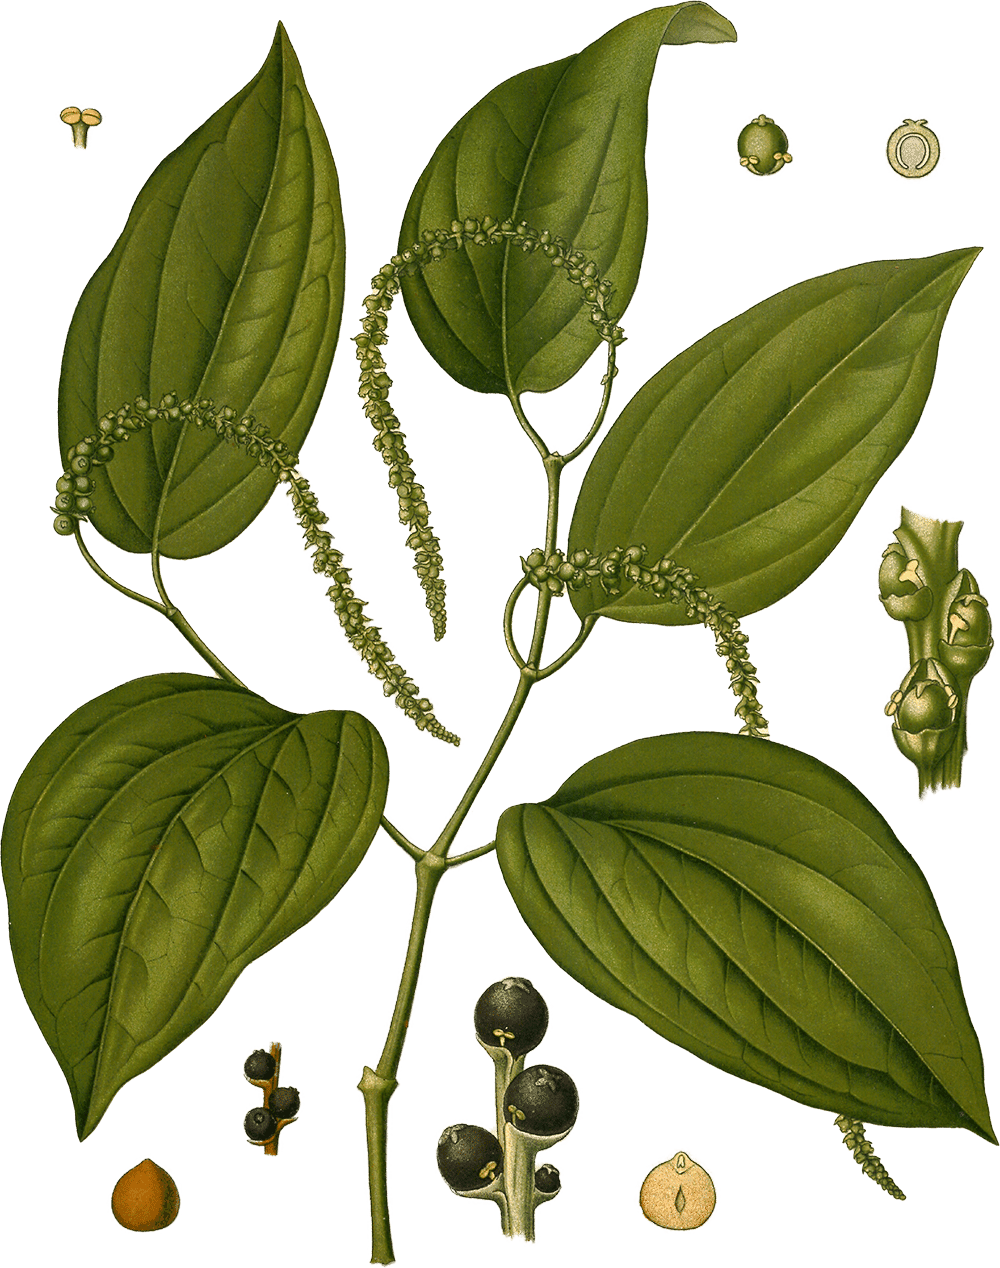
\includegraphics[width=\linewidth]{imgs/pepper.pdf}
%     \caption{Etymology of the English word \textit{pepper}, and an illustration of its approximate route.}
%     \label{map:pepper_etymology}
% \end{figure}

